\documentclass[a4paper, 11pt, notitlepage, english]{article}

\usepackage{babel}
\usepackage[utf8]{inputenc}
\usepackage[T1]{fontenc, url}
\usepackage{textcomp}
\usepackage{amsmath, amssymb}
\usepackage{amsbsy, amsfonts}
\usepackage{graphicx, color, xcolor}
\usepackage{verbatim, listings, fancyvrb}
\usepackage{parskip}
\usepackage{framed}
\usepackage{amsmath}
\usepackage{multicol}
\usepackage{url}
\usepackage{flafter}
\usepackage{simplewick}
\usepackage{amsthm}
\usepackage{bbold}


\usepackage{caption}
\DeclareCaptionLabelSeparator{colon}{. }
\renewcommand{\captionfont}{\small\sffamily}
\renewcommand{\captionlabelfont}{\bf\sffamily}
\usepackage{float}
%\floatstyle{ruled}
%\restylefloat{figure}
\setlength{\captionmargin}{20pt}
%\addto\captionsenglish{\renewcommand{\figurename}{Fig.}}
\usepackage{bigstrut}
\setlength{\tabcolsep}{12pt}


\newtheorem{theorem}[]{Wick's Theorem}[]

\DeclareUnicodeCharacter{00A0}{~}

\definecolor{javared}{rgb}{0.6,0,0} % for strings
\definecolor{javagreen}{rgb}{0.25,0.5,0.35} % comments
\definecolor{javapurple}{rgb}{0.5,0,0.35} % keywords
\definecolor{javadocblue}{rgb}{0.25,0.35,0.75} % javadoc

\lstset{language=python,
basicstyle=\ttfamily\scriptsize,
keywordstyle=\color{javapurple},%\bfseries,
stringstyle=\color{javared},
commentstyle=\color{javagreen},
morecomment=[s][\color{javadocblue}]{/**}{*/},
morekeywords={super, with},
% numbers=left,
% numberstyle=\tiny\color{black},
stepnumber=2,
numbersep=10pt,
tabsize=2,
showspaces=false,
captionpos=b,
showstringspaces=false,
frame= single,
breaklines=true}

\usepackage{geometry}
\geometry{headheight=0.01mm}
\geometry{top=20mm, bottom=20mm, left=34mm, right=34mm}

\renewcommand{\arraystretch}{2}
\setlength{\tabcolsep}{10pt}
\makeatletter
\renewcommand*\env@matrix[1][*\c@MaxMatrixCols c]{%
  \hskip -\arraycolsep
  \let\@ifnextchar\new@ifnextchar
  \array{#1}}
%
% Definering av egne kommandoer og miljøer
%
\newcommand{\dd}[1]{\ \text{d}#1}
\newcommand{\f}[2]{\frac{#1}{#2}} 
\newcommand{\beq}{\begin{equation}}
\newcommand{\eeq}{\end{equation}}
\newcommand{\bra}[1]{\langle #1|}
\newcommand{\ket}[1]{|#1 \rangle}
\newcommand{\braket}[2]{\langle #1 | #2 \rangle}
\newcommand{\brakket}[2]{\langle #1 || #2 \rangle}
\newcommand{\braup}[1]{\langle #1 \left|\uparrow\rangle\right.}
\newcommand{\bradown}[1]{\langle #1 \left|\downarrow\rangle\right.}
\newcommand{\av}[1]{\left| #1 \right|}
\newcommand{\op}[1]{\hat{#1}}
\newcommand{\braopket}[3]{\langle #1 | {#2} | #3 \rangle}
\newcommand{\ketbra}[2]{\ket{#1}\bra{#2}}
\newcommand{\pp}[1]{\frac{\partial}{\partial #1}}
\newcommand{\ppn}[1]{\frac{\partial^2}{\partial #1^2}}
\newcommand{\up}{\left|\uparrow\rangle\right.}
\newcommand{\upup}{\left|\uparrow\uparrow\rangle\right.}
\newcommand{\down}{\left|\downarrow\rangle\right.}
\newcommand{\downdown}{\left|\downarrow\downarrow\rangle\right.}
\newcommand{\updown}{\left|\uparrow\downarrow\rangle\right.}
\newcommand{\downup}{\left|\downarrow\uparrow\rangle\right.}
\newcommand{\bupup}{\left.\langle\uparrow\uparrow\right|}
\newcommand{\bdowndown}{\left.\langle\downarrow\downarrow\right|}
\newcommand{\bupdown}{\left.\langle\uparrow\downarrow\right|}
\newcommand{\bdownup}{\left.\langle\downarrow\uparrow\right|}
\renewcommand{\d}{{\rm d}}
\newcommand{\Res}[2]{{\rm Res}(#1;#2)}
\newcommand{\To}{\quad\Rightarrow\quad}
\newcommand{\eps}{\epsilon}
\newcommand{\inner}[2]{\langle #1 , #2 \rangle}
\renewcommand{\u}{\uparrow}
\renewcommand{\d}{\downarrow}
\newcommand{\dddd}{\d\d\d\d}
\newcommand{\uddd}{\u\d\d\d}
\newcommand{\dudd}{\d\u\d\d}
\newcommand{\ddud}{\d\d\u\d}
\newcommand{\dddu}{\d\d\d\u}
\newcommand{\uudd}{\u\u\d\d}
\newcommand{\udud}{\u\d\u\d}
\newcommand{\uddu}{\u\d\d\u}
\newcommand{\duud}{\d\u\u\d}
\newcommand{\dudu}{\d\u\d\u}
\newcommand{\dduu}{\d\d\u\u}
\newcommand{\uuud}{\u\u\u\d}
\newcommand{\uudu}{\u\u\d\u}
\newcommand{\uduu}{\u\d\u\u}
\newcommand{\duuu}{\d\u\u\u}
\newcommand{\uuuu}{\u\u\u\u}
\newcommand{\m}{\text{-}}
\newcommand{\ui}{{\u_1}}
\newcommand{\uii}{{\u_2}}
\newcommand{\uiii}{{\u_3}}
\newcommand{\di}{{\d_1}}
\newcommand{\dii}{{\d_2}}
\newcommand{\diii}{{\d_3}}

\newenvironment{psmallmatrix}
  {\left(\begin{smallmatrix}}
  {\end{smallmatrix}\right)}

\newenvironment{bsmallmatrix}
  {\left[\begin{smallmatrix}}
  {\end{smallmatrix}\right]}



\newcommand{\bt}[1]{\boldsymbol{#1}}
\newcommand{\mat}[1]{\textsf{\textbf{#1}}}
\newcommand{\I}{\boldsymbol{\mathcal{I}}}
\newcommand{\p}{\partial}
%
% Navn og tittel
%
\author{Jonas van den Brink \\ \texttt{j.v.brink@fys.uio.no}}
\title{Beam Optics \\ A Lab report in FYS4180}


\begin{document}
\maketitle

\vspace{1cm}

\tableofcontents

\clearpage

\section{Title}

... of near-gaussian beams

Computing and measuring the divergence of near-gaussian beams

\clearpage

\section{Abstract}
A laser beam with a gaussian transverse intensity distribution can be characterized mainly by two quantities, the width of the beam and the radius of curvature. The evolution of these quantities over time can be computed using ray transfer matrix formalism. 

In beam optics, one of the main goals is to manipulate a laser beam, this is frequently done by letting the beam pass through various optical devices, such as lenses, filters, mirrors and so on. Such optical devices affect the laser beam through diffraction, altering the radius of curvature and width of the laser beam.

In this report we start by giving a short introduction to beam optics and ray transfer matrix formalism. The assumptions that underlie our calculations are covered in details.

Next we turn to experimental beam optics, by setting up an experimental configuration in the optics lab. Here, we measure the development of a laser beam over a distance of a few meters. We then insert lenses into the path of the beam and measure how the laser beam is changed. The lab measurements are compared to formal calculations and a parameter-optimiziation scheme is used to find the radius of curvature of the laser beam.

Thereafter we turn to a long-distance measurement, where we let the laser beam travel about a kilometer before the width of the beam is measured. We then insert lenses at the origin of the beam to attempt to minimize the width of the beam at the target.




\clearpage

\section{Theory}

\subsection{Gaussian Beams}



When a Gaussian beam travels undisturbed through a vacuum, it will behave in a well-known manner. A sketch is shown in figure \ref{fig:gaussian_beam}. If the beam has a negative radius of curvature, it will narrow until it reaches a minimum where the radius of curvature becomes positive and the beam again begins to expand. The point where the beam is the narrowest is often referred to as the \emph{waist} of the beam. We denote the width of the beam at the waist as $w_0$. The distance from the waist to the point where the area of the beam has doubled is reffered to as the \emph{Rayleigh range}, $Z_{\rm R}$. The beam is symmetric around its waist, meaning we can move $Z_R$ to either direction from the waist, and the width of the beam will be $\sqrt{2}w_0$. If we move much further than the Rayleigh range away from the waist, the width of the beam will increase linearily. The angle formed between the optical axis and the beam far from the waist is called the divergence of the beam, which we will denote $\theta$.

\begin{figure}[htpb]
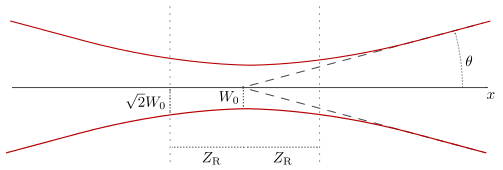
\includegraphics[width=\textwidth]{beam.pdf}	
\caption{Sketch of how a Gaussian beam changes when close to its minimum width. \label{fig:gaussian_beam}}
\end{figure}

It can be shown that the divergence of a Gaussian beam is
$$\theta = \frac{\lambda}{\pi w_0}.$$


"I moderne optikk benyttes ofte lasterstråler med gaussisk intensitetsfordeling på tvers av strålen. Da vil stråleformen beholdes selv etter at strålen stadig er gjenstand for diffraksjon."

At en lasterstråle har gaussisk intensitetsprofil er en forutsetning for å behandle


From the waist we can move a given distance in either direction until the beam has doubled in area, meaning the width is 

If we move a distance $\sqrt{2}w_0$, which is known as the Rayleigh length, away from the waist, the area of the beam will





Vistnes claims that one often uses gaussian beams in modern optics, as such a beam will maintain its beamprofile, even after repeated diffractions.


When a beam is refracted through a lens, the parameters of the Gaussian beam may be changed, but the Guassian beam profile itself is maintained.

For a gaussian beam, we also have a well-defined measure of the width of the beam, it is the value where the intensity has fallen to $1/e^2$ of the peak.

The two main quantities in the formalism is the beam diameter and radius of curvature.

"Because the divergence is inversely proportional to the spot size, a Gaussian beam that is focused to a small spot spreads out rapidly as it propagates away from that spot. To keep a laser beam very well collimated, it must have a large diameter. This relationship between beam width and divergence is due to diffraction. Non-Gaussian beams also exhibit this effect, but a Gaussian beam is a special case where the product of width and divergence is the smallest possible.
"

\subsection{Tansfer Matrix Analysis}




\subsubsection{Ray Transfer Matrix Analysis}

The path of a ray is usually classified by the position

\subsubsection{The Beam Parameter}

The transfer matrix analysis formalism cannot readily be used for a laser beam, as beam formalism presupposes that any beam has a given width which needs to be classified. However, a complex beam parameter can be introduced
$$\frac{1}{q} = \frac{1}{R} - \frac{i\lambda}{\pi n w^2},$$
where $R$ is the radius of curvature and $w$ is the beam spot size, i.e., the width of the beam. With the introduction of this beam parameter, we can define a \emph{beam}-vector, which is simply $(q,1)$. With the introduction of this beam-vector, we can use the transfer matrix analysis also for beams. When multiplying a beam-vector with a given RTM, the second component of the beam-vector might change, we therefore introduce a \emph{renormalization-constant}, $k$, which holds the second component of the beam-vector at unity.

\subsection{Optical devices}

\subsubsection{Lenses}

A lens is a transmissive optical device, meaning light passes through it. The light that passes through a lens is changed due to diffraction. Many different lenses can be built, but we will limit our discussion to simple biconcave and biconvex lenses.

\begin{figure}[htpb]
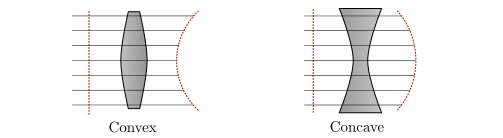
\includegraphics[width=\textwidth]{lenses.pdf}	
\caption{Sketch of the optical path of the different parts of a beam that passes through an abstract lens. \label{fig:lenses}}
\end{figure}

An abstract, idealized lens only changes the radius of curvature $R$ of the beam that passes through it. To understand how the curvature is changed, it is helpful to think of the optical path of different parts of the beam. Figure \ref{fig:lenses} shows schematically a beam pasing through a biconvex and a biconcave lens. As a lens is generally made of a material with a higher index of refraction than air, light passes through the lens slower than in the air. This means that the parts of the beam that passes through the thinnest parts of the lens can move further away from the lens than the the parts of the beam that has to pass through the thickest part of the lens. 

If we then draw a virtual line through the parts of the beam with the same phase after it has passed through the lens, we see how the curvature has been affected. Assuming the beam had a completely planar curvature before the lens, a convex lens will change the curvature to a positive one, while the concave lens will make it negative. More specifically, the curvature will be equal to focal length of the lens.

As should be apparent, the situtation shown in figure \ref{fig:lenses} does not require the beam to pass from left-to-right. The lenses are symmetrical and so the light could just as easily move from right-to-left. This means that a beam which has a curvature equal to the focal length of a lens will be turned into a planar wave by passing through that lens. We use this fact when we construct a beam expander.

\subsubsection{Beam Expanders and Narrowers} \label{sec:beam_expander}

The goal of a beam expander is to increase the width of a beam without changing it's radius of curvature. Such a device can be made in different ways, but let us look at a simple setup using two biconvex lenses. A sketch of a possible setup is shown in figure \ref{fig:beam_expander}

\begin{figure}[htpb]
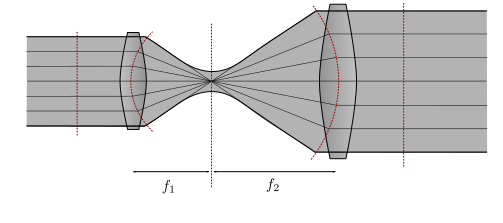
\includegraphics[width=\textwidth]{beam_expander.pdf}	
\caption{Sketch of a beam passing through a beam expander made from two biconvex lenses. \label{fig:beam_expander}}
\end{figure}

If we assume a planar beam hits a convex lens the curvature will become positive, this is explained in the previous section. Due to the curvature of the beam, it will narrow as it continues after the lens, hitting it's minimum width at the focal length of the lens. After passing the minimum it will expand again, meaning the curvature has become negative. If we place another convex lens at the right distance the beam can again become planar by passing through it. For this to happen, the lens has to be placed so that the distance from the waist to the lens is preciesly equal to it's focal length. The net result is that a planar wave has been expanded without any alteration in the curvature. 

Just as in the previous example, there is no preference for the beam to pass from left-to-right in the sketch, meaning we can just as easily create a \emph{beam narrower} from two biconvex lenses. The difference between the expander and narrower is simply which lens has the biggest focal length. If the first lens has a smaller focal length, i.e., $f_1 < f_2$ the beam is expanded and vice versa.

\clearpage

\section{Experiments}

\subsection{Finding the Radius of Curvature of a beam}

The first experiment we conducted in the lab had the goal of finding the radius of curvature of a laser beam. 

\subsubsection{Method}

This experiment was conducted using a Helium-Neon (HeNe) laser as our beam source. The laser itself generated a beam of a constant, non-adjustable, intensity. The  beam was therefore passed through an optical setup that let us adjust the intensity of the resulting beam. A picture of the optical setup is shown in figure \ref{fig:setup_photo} and a sketch of the setup is shown in figure \ref{fig:setup_sketch}.

\begin{figure}[p]
\includegraphics[width=\textwidth, angle=180]{oppsett_photo}	
\caption{Photo of the optical setup. After being reflected in the mirror on the right-hand side on the picture, the beam travels a measured distance before hitting a beam profiler which measures the transversal intensity of the beam. \label{fig:setup_photo}}
\end{figure}

\begin{figure}[p]
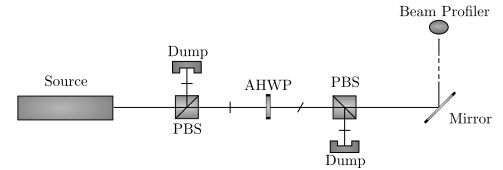
\includegraphics[width=\textwidth]{oppsett1}	
\caption{Sketch of the optical setup. The laser beam passes from the source through a polarizing beam splitter (PBS). Roughly half of the light is then reflected and passed to a dump, the transmitted light will be linearily polarized along a given axis. Next the linearily polarized light passes through an adjustable half wave plate (AHWP), which rotates the polarization-plane. Next, the beam passes through another PBS and the reflection is again captured by a dump. The amount of light that is now reflected depends on how much the polarization has been rotated by the AHWP. The transmitted part of the beam is reflected by a mirror and travels a measured distance before hitting a beam profiler, which measures the transversal intensity of the beam. \label{fig:setup_sketch}}
\end{figure}

\clearpage

\subsubsection{Results}
\subsubsection{Discussion}

\subsection{Measuring the effects of a Beam Expander}

We now use the same experimental set up as in the last section, but now we let the beam pass through a beam expander, we will study how the beam is affected by the beam expander and how this changes if we make small adjustment to the distance between the two lenses which compromise the beam expander.

\subsubsection{Method}

As before, we have a biconvex lens with a focal length $f_1 = 100$ mm positioned at $200$ mm, we introduce another biconvex lens at $500 mm$, this with a focal length of $f_2=200$ mm. As the first lens has a smaller focal length than the second, and the distance between the lenses is equal the the sum of the focal lengths, the two lenses make a beam expander, as explained in section \ref{sec:beam_expander}.

Letting the lens at 200 mm remain, we introduce a new biconvex lens at 500 mm. This means that the first lens has a focal length $f_1=100$ mm and the second lens has a focal length $f_2=200$ mm. The beam that enters the beam expander in our experimental setup is definitly \emph{not} a perfectly plane wave, so we will have to adjust the distance between the beam expanders slightly to calibrate our beam expander.

\subsubsection{Results}
\subsubsection{Discussion}

\subsection{Long-distance measurements of a laser beam}
\subsubsection{Method}
\subsubsection{Results}
\subsubsection{Discussion}

\clearpage

\section{Theoretical Calculations}

\clearpage

\section{Conclusions}



\begin{figure}[htpb]
\includegraphics[width=\textwidth]{fig1.pdf}	
\caption{Observed width of the laser beam at different distances and the best-fit RTMA curve as found by the least-squared method.}
\end{figure}





\clearpage


\section{Sources} 

[1] Vistnes, Arnt-Inge, 2013. \emph{Svingninger og bølger}. Digitale utgivelser ved UiO.

\url{http://en.wikipedia.org/wiki/M_squared}

\url{http://en.wikipedia.org/wiki/Diffraction}

\url{http://en.wikipedia.org/wiki/Ray_transfer_matrix_analysis#Ray_transfer_matrices_for_Gaussian_beams}

\url{http://en.wikipedia.org/wiki/Gaussian_beam}

\url{http://en.wikipedia.org/wiki/Beam_parameter_product}
\section{}






\end{document}